Viscosity is a property of fluids (liquids and gases) which determines how much resistance is experienced by an object trying to move through the fluid. In this experiment we will use Stoke's Law and the concept of terminal velocity to determine the viscosity of glycerin.

\section*{Objective}

   Use Stoke's Law to derive an equation relating the viscosity $\eta$ of a fluid to the time $t$ it takes for a sphere to fall a distance $d$ through it.

\section*{Experimental Setup}

   The equipment consists of a long glass cylinder filled with glycerin. A graduated scale is attached to the cylinder which allows us to measure distances along the cylinder.
   
   Small metallic spheres are dropped from the top of the cylinder. The viscosity of the glycerin produces a drag force that will eventually result in terminal velocity being achieved by the falling sphere. The terminal velocity is calculated by measuring the time $t$ it takes the sphere to fall through a distance $d$ inside the fluid.

   \tikzsetnextfilename{setup}
\begin{center}
   \begin{tikzpicture}

      \usetikzlibrary{patterns}
      % We define a tikz style which defines a fill pattern consisting of lines in the north east direction.
      % The draw=none option indicates that we do NOT want any stroke/border around the fill
      \tikzstyle{wall}=[fill,pattern=north east lines,minimum width=0.75cm,minimum height=0.3cm, draw=none]


      % Define dimensions and angles
      \def\hw{0.25}     % Half width of the small wall segment on top

      \def\angle{-120}  % Angle of string
      \def\r{5}         % Radius of string

      \def\br{0.1}      % Radius of bob


      % Draw commands
      \draw (-\hw, 0) -- (\hw, 0);
      \draw [wall] (-\hw,0) rectangle (\hw,0.1);        % Draws a rectangle using the 'wall' pattern giving us the sloped lines

      \draw (0,0) -- (\angle:\r);       % string
      \draw [dashed] (0,0) -- (0,-\r);  % Dashed line down the middle

      \draw (\angle:\r+\br) circle [radius=\br];
      
   \end{tikzpicture}
\end{center}


\section*{Free-Body Diagram}

   A sphere falling through a fluid experiences three forces: its weight $W$, an upward buoyant force $F_B$ (Archimedes' Principle) and the drag force $F_D$ (Stoke's Law) also in the upward direction since it opposes the downward motion of the sphere.

   \tikzsetnextfilename{freebody}      % We set the filename which will be used for the pdf created by the externalize library. The prefix is still applicable so build/freebody.pdf will be created
\begin{center}
   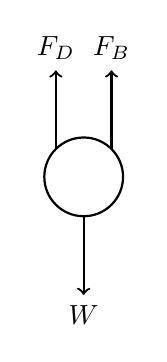
\begin{tikzpicture}

      \def\r{0.5}
      \def\h{1}

      \draw 
         (0,0) [thick] circle [radius=\r];

      \draw [thick] (0, -\r) [->] -- ++ (0,-\h) node [below] {$W$};

      \draw [thick] (45:\r) [->] -- ++ (0, \h) node [above] {$F_B$};

      \draw [thick] (135:\r) [->] -- ++ (0, \h) node [above] {$F_D$}; 

   \end{tikzpicture}
\end{center}


\section*{Derivation}

   The three forces acting on the falling sphere are given by
   \beqc \label{three_forces}
      W = m g\\
      F_B = \sigma \, V g\\
      F_D = 6 \pi \, \eta \, r v\\
   \eeqc
   where $\sigma$ is the density of the fluid and the last equation is a statement of Stoke's Law which describes the drag force acting on a sphere of radius $r$ as it moves with velocity $v$ through a fluid with viscosity $\eta$.

   The first two forces remain constant but the drag force increases in magnitude as the sphere speeds up since it is directly proportional to the velocity $v$. Initially, when the velocity of the sphere is low, the drag force is low as well and therefore the net downward force and acceleration are large. This causes the velocity to increase. As the velocity increases the drag force increases and in turn the net downward force and acceleration decrease. The velocity keeps increasing but at a slower rate. Eventually the drag force increases until it exactly balances the other two forces. The net downward force and acceleration become zero and the velocity becomes constant. This is known as the terminal velocity $v_T$.

   Therefore, by definition, when the terminal velocity is achieved the net force on the sphere is zero, the three forces balance each other out. Looking at the free-body diagram this means
   \beq
      W = F_B + F_D
   \eeq
   \def\stokes{6 \pi \, \eta \, r v_T}

   Substituting \eqref{three_forces}
   \beqn
      \imply m g = \sigma \, V g + \stokes 
   \eeqn

   The mass of the sphere $m$ can be expressed in terms of the density $\rho$ of the sphere as $m = \rho V$.
   \beqcn
      \imply \rho V g = \sigma \, V g + \stokes\\
      \imply \stokes = \rho V g - \sigma V g\\
      \imply \stokes = (\rho - \sigma) V g
   \eeqcn

   The volume of a sphere is given by $V = \frac{4}{3} \pi r^3$. If the sphere (after attaining terminal velocity) falls through a distance $d$ in time $t$ the terminal velocity can be calculated using $v_T = \frac{d}{t}$. Substituting these in
   \beqcn
      \imply 6 \pi \, \eta \, r \frac{d}{t} = (\rho - \sigma) \frac{4}{3} \pi r^3 g\\
      \imply 3 \, \eta \, \frac{d}{t} = \frac{2}{3} (\rho - \sigma) g \, r^2\\
   \eeqcn

   Since our aim is to calculate the viscosity of the fluid we make $\eta$ the subject of the equation giving us

   \beq
      \eta = \frac{2}{9} \frac{(\rho - \sigma) g \, r^2 t}{d}
   \eeq

   Thus we end up with an equation that relates the viscosity of a fluid to the radius of the sphere falling through it and the time it takes for it to fall through a certain distance. This equation governs the working of a \textbf{viscometer} a device where falling spheres are used to measure the viscosity of a fluid.
